
\chapter{Składanie dokumentu w systemie \LaTeX}

To jest tylko przykład załączników - jak się domyslam

W tym rozdziale znajduje się
garść informacji o tym, jak poprawnie składać tekst pracy w systemie \LaTeX{} wraz z 
przykładami, które mają służyć do przeklejania do własnych dokumentów.

\section{Struktura dokumentu}
\chaptermark{Tytuł rozdziału, jeśli pełen się nie mieści\ldots{}}{}

Praca składa się z rozdziałów (\texttt{chapter}) i podrozdziałów (\texttt{section}).
Ewentualnie można również rozdziały zagnieżdzać (\texttt{subsection}, \texttt{subsubsection}),
jednak nie powinno się wykraczać poza drugi poziom hierarchii (czyli \texttt{subsubsection}).

\section{Akapity i znaki specjalne}

Akapity rozdziela się od siebie przynajmniej jedną pustą linią. Podstawowe
instrukcje, które się przydają to \emph{wyróżnienie pewnych słów}. Można również
stosować \textbf{styl pogrubiony}, choć nie jest to generalnie zalecane.

Należy pamiętać o zasadach polskiej interpunkcji i ortografii. Po spójnikach 
jednoliterowych warto wstawić znak tyldy ($\sim$), który jest tak zwaną
,,twardą spacją'' i powoduje, że wyrazy nią połączone nie będą rozdzielane
na dwie linie tekstu.

Polskie znaki interpunkcyjne różnią się nieco od angielskich: to jest ,,polski'', a to jest
``angielski''. W kodzie źródłowym tego tekstu będzie widać różnicę.

Proszę również zwrócić uwagę na znak myślnika, który może być pauzą ,,---'' lub
półpauzą: ,,--''. Należy stosować je konsekwentnie. Do łączenia wyrazów używamy
zwykłego ,,-'' (\emph{północno-wschodni}), do myślników --- pauzy lub półpauzy.
Inne zasady interpunkcji i typografii można znaleźć w słownikach.

\section{Wypunktowania}

Wypunktowanie z cyframi:
\begin{enumerate}
    \item to jest punkt,
    \item i to jest punkt,
    \item a to jest ostatni punkt.
\end{enumerate}

\noindent
Po wypunktowaniach czasem nie warto wstawiać wcięcia akapitowego. Wtedy przydatne jest
polecenie \texttt{noindent}. Wypunktowanie z kropkami (tzw.~\emph{bullet list}) wygląda tak:
\begin{itemize}
    \item to jest punkt,
    \item i to jest punkt,
    \item a to jest ostatni punkt.
\end{itemize}

\noindent
Wypunktowania opisowe właściwie niewiele się różnią:
\begin{description}
    \item[elementA] to jest opis,
    \item[elementB] i to jest opis,
    \item[elementC] a to jest ostatni opis.
\end{description}


\section{Polecenia pakietu \texttt{ppfcmthesis}}

Parę poleceń zostało zdefiniowanych aby uspójnić styl pracy. Są one przedstawione poniżej
(oczywiście nie trzeba się do nich stosować).

\paragraph{Makra zdefiniowane dla języka angielskiego.} Są nimi: \texttt{termdef} oraz \texttt{acronym}.
Przykłady poniżej obrazują ich przewidywane użycie w tekście.
\begin{center}\footnotesize%
\begin{tabular}{l >{\rightskip\fill}p{12cm}}
\toprule
źródło   & \texttt{we call this a $\backslash$termdef\{Database Management System\} ($\backslash$acronym\{DBMS\})} \\ \cmidrule(lr){2-2}
docelowo & we call this a \termdef{Database Management System} (\acronym{DBMS}) \\ 
\bottomrule
\end{tabular}
\end{center}

\paragraph{Makra zdefiniowane dla języka polskiego.} Podobnie jak dla języka angielskiego zdefiniowano
odpowiedniki polskie: \texttt{defini\-cja}, \texttt{akronim} oraz \texttt{english} dla tłumaczeń angielskich
terminów. Przykłady poniżej obrazują ich przewidywane użycie w tekście.
\begin{center}\footnotesize%
\begin{tabular}{l >{\rightskip\fill}p{12cm}}
\toprule
źródło   & \texttt{nazywamy go $\backslash$definicja\{systemem zarządzania bazą danych\} ($\backslash$akronim\{DBMS\}, $\backslash$english\{Database Management System\})} \\ \cmidrule(lr){2-2}
docelowo & nazywamy go \definicja{systemem zarządzania bazą danych} (\akronim{DBMS}, \english{Database Management System}) \\ \bottomrule
\end{tabular}
\end{center}


\section{Rysunki}

Wszystkie rysunki (w tym również diagramy, szkice i inne) osadzamy w środowisku 
\texttt{figure} i umieszczamy podpis \emph{pod} rysunkiem, w formie elementu \texttt{caption}. Rysunki powinny
zostać umieszczone u góry strony (osadzone bezpośrednio w treści strony zwykle utrudniają czytanie tekstu).
Rysunek~\ref{rys:plama} zawiera przykład pełnego osadzenia rysunku na stronie.

\begin{figure}[t] % możliwe opcje to 't' - top, 'b' - bottom, 'h' - 'here', ale zaleca się 't'
\centering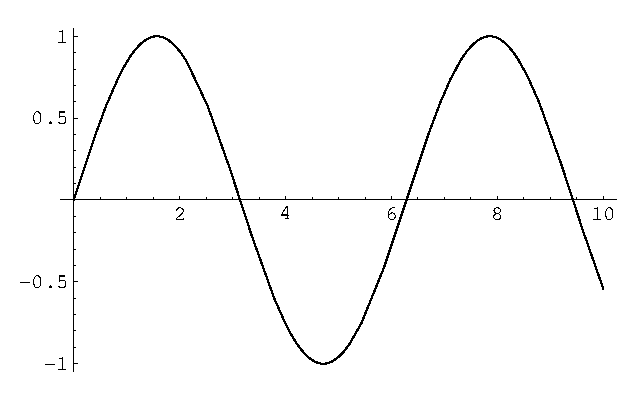
\includegraphics[width=5cm]{figures/mathematica}
\caption{Wykres.}\label{rys:plama}
\end{figure}

\begin{figure}[t]
\centering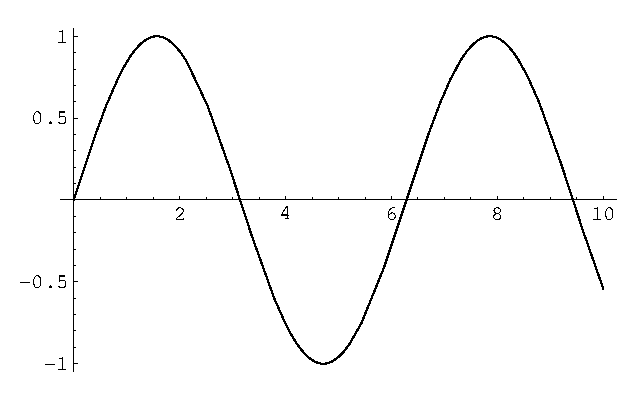
\includegraphics[width=\textwidth]{figures/mathematica}
\fcmfcaption{Ten sam wykres ale na szerokość tekstu. Formatowanie podpisu zgodne z wytycznymi FCMu.}\label{rys:plama2}
\end{figure}

Styl FCMu to nieco inne nagłówki rysunków. Dostepne są one poleceniem \texttt{fcmfcaption} (zob.~rysunek
\ref{rys:plama2}).

\subsection{Tablice}

Tablice to piękna rzecz, choć akurat ich umiejętne tworzenie w \LaTeX{}u nie jest łatwe. 
Jeśli tablica jest skomplikowana, to można ją na przykład wykonać w programie
OpenOffice, a następnie wyeksportować jako plik \akronim{PDF}. W każdym przypadku tablice wstawia się podobnie
jak rysunki, tylko że w środowisko \texttt{table}. Tradycja typograficzna sugeruje umieszczenie opisu tablicy, a więc
elementu \texttt{caption} ponad jej treścią (inaczej niż przy rysunkach).  

Tablica~\ref{tab:tabela} pokazuje pełen przykład.

\begin{table}[ht]
\caption{Przykładowa tabela. Styl opisu jest zgodny z rysunkami.}\label{tab:tabela}
\centering\footnotesize%
\begin{tabular}{l c}
\toprule
artykuł & cena [zł] \\
\midrule
bułka   & $0,4$ \\
masło   & $2,5$ \\
\bottomrule
\end{tabular}
\end{table}

Zasady FCMu sugerują nieco inne nagłówki tablic. Dostepne są one poleceniem \texttt{fcmtcaption} (zob.~tablicę
\ref{tab:tabela2}).

\begin{table}[ht]
\fcmtcaption{Przykładowa tabela. Styl opisu jest zgodny z wytycznymi FCMu.}\label{tab:tabela2}
\centering\footnotesize%
\begin{tabular}{l c}
\toprule
artykuł & cena [zł] \\
\midrule
bułka   & $0,4$ \\
masło   & $2,5$ \\
\bottomrule
\end{tabular}
\end{table}


\subsection{Checklista}

\begin{itemize}
\item Znakiem myślnika jest w LaTeXu dywiz pełen (---) albo półpauza (--), przykład:
  A niech to jasna cholera --- wrzasnąłem.

\item Połączenie między wyrazami to zwykły myślnik, przykład:   północno-zachodni

\item Sprawdź czy tutuł pracy ma maksymalnie dwa wiersze i czy stanowią one pełne frazy
  (czy nie ma przeniesienia bez sensu).

\item Sprawdź ostrzeżenia o 'overfull' i 'underful' boxes. Niektóre z nich można zignorować (spójrz
  na wynik formatowania), niektóre trzeba poprawić; czasem przeformułować zdanie.

item Przypisy stawia się wewnątrz zdań lub za kropką, przykład:
  Footnote is added after a comma.\footnote{Here is a footnote.}

\item Nie używaj przypisów zbyt często. Zobacz, czy nie lepiej będzie zintegrować przypis z tekstem.

\item Tytuły tabel, rysunków powinny kończyć się kropką.

\item Nie używaj modyfikatora [h] (here) do rysunków i tabel. Rysunki i tabele powinny być
  justowane do góry strony lub na stronie osobnej.

\item Wyróżnienie w tekście to polecenie \emph{wyraz}, nie należy używać czcionki pogrubionej (która
  wystaje wizualnie z tekstu i rozprasza).

\item Nazwy plików, katalogów, ścieżek, zmiennych środowiskowych, klas i metod formatujemy poleceniem
  \texttt{plik\_o\_pewnej\_nazwie}.

\item Po ostatniej zmianie do treści, sprawdź i przenieś wiszące spójniki wstawiając przed nie znak
  tyldy (twardej spacji), przykład:
  Ala i~kotek nie lubią mleczka, a~Stasiu lubi.
  
\item Za i.e. (id est) i e.g. (exempli gratia) stawia się zwyczajowo przecinek w typografii amerykańskiej.

\item Przed i za pełną pauza nie ma zwyczajowo spacji w typografii amerykańskiej, przykład:
  Darn, this looks good---said Mary.

\item Zamykający cudzysłów oraz footnote wychodzą za ostatni znak interpunkcji w typografii 
  amerykańskiej, przykłady:
  It can be called a ``curiosity,'' but it's actually normal.
  Footnote is added after a comma.\footnote{Here is a footnote.}

\item Odwołania do tabel i rysunków zawsze z wielkiej litery, przykład:
  In Figure~\ref{rys:plama} we illustrated XXX and in Table~\ref{tab:tabela} we show detailed data.
  
\end{itemize}


\section{Literatura i materiały dodatkowe}

Materiałów jest mnóstwo. Oto parę z nich:
\begin{itemize}
    \item \emph{The Not So Short Introduction\ldots}, która posiada również tłumaczenie 
    w języku polskim.\\
    \url{http://www.ctan.org/tex-archive/info/lshort/english/lshort.pdf}

    \item Klasy stylu \texttt{memoir} posiadają bardzo wiele informacji o składzie tekstów
    anglosaskich oraz sposoby dostosowania \LaTeX{}a do własnych potrzeb.\\
    \url{http://www.ctan.org/tex-archive/macros/latex/contrib/memoir/memman.pdf}
    
    \item Nasza grupa dyskusyjna i repozytorium Git są również dobrym miejscem aby zapytać
    (lub sprawdzić czy pytanie nie zostało już zadane).\\
    \url{https://github.com/politechnika/put-latex}

    \item Dla łaknących więcej wiedzy o systemie LaTeX podstawowym źródłem informacji
    jest książka Lamporta~\cite{Lamport1985}. Prawdziwy \emph{hardcore} to oczywiście
    \emph{The \TeX{}book} profesora Knutha~\cite{Knuth1986}.
\end{itemize}

